%==============================================================================
%  MATH 231 -- Linear Algebra I (Queens College, Fall 2026)
%  PROJECT 1 -- Neighbours, Clusters, and Valleys
%
%  WHAT IT IS.  A Python project with three self-contained choices.  Each
%  student completes ONE choice -- names it with TRACK at the top of project1.py
%  -- and writes the report for that choice only.  Each choice ends in a picture or
%  an animation, and each closes with its own report questions:
%     Choice 1  (TRACK "knn")      k-nearest neighbours on a 2-D song data set
%             (duration, energy), with the feature-scaling lesson built in: raw
%             accuracy is ~45% (chance is 33%), standardized accuracy ~90%.
%     Choice 2  (TRACK "kmeans")   k-means (Lloyd) on 320 customer locations in
%             four neighbourhoods ("park four food trucks"): a deliberately bad
%             start that sticks at J = 1086.27, ten random restarts (one of
%             which sticks the same way), and an elbow plot with its elbow at
%             k = 4.
%     Choice 3  (TRACK "descent")  gradient descent on
%             f(x,y) = sin x cos y + 0.08 (x^2 + y^2), which has EIGHT valleys
%             with floors inside [-6,6]^2 (depths -0.830, -0.153 twice, 0.523,
%             1.164 twice, 1.841 twice), animated live on the 3-D surface and a
%             contour map; a learning-rate table; and a start where eta = 1.5
%             hops into the deepest valley that eta = 0.1 misses.  A ninth local
%             minimum at (-6.246, 0) lies just outside the window.
%
%  ONE CHOICE EACH.  runproject1.py runs only the choice TRACK names (the grader
%  runs it with no arguments), so the graded output is exactly one choice.  A
%  student can still try another choice with "python runproject1.py kmeans" and
%  so on, or "all".  If TRACK is unset or misspelt, runproject1.py runs all three
%  choices and prints a reminder to set it.  play.py likewise plays only the
%  selected choice's animations; Choice 1 has none.
%
%  GRADING.  Every choice is out of 100: code 55, report 45.  The code points
%  are split by function within each choice (the table in "How it is graded");
%  the report is R1-R2 at 18 points each plus the limits paragraph at 9.  Both
%  the 55/45 split and the per-function weights are a proposal.
%
%  LECTURES IT RESTS ON.  Computational unit Part 2 (k-NN, Sec. 5-10), Part 3
%  (k-means, Sec. 11-15) and Part 6 (gradient descent, Sec. 24-27); vector unit
%  Sec. 14 (metrics); vector calculus unit Sec. 6-7 (partial derivatives,
%  gradient) and Sec. 8 (steepest ascent).  AS OF OCT 1 NONE OF THE THREE
%  COMPUTATIONAL-UNIT LECTURES HAD BEEN GIVEN (README recap table), and vector
%  calculus stopped at Sec. 7.  The syllabus says projects implement "an
%  algorithm already developed in lecture", so either assign this after those
%  lectures, or rely on the fact that every algorithm is stated in full in a
%  box below and the handout is self-contained.  With one choice per student,
%  it is also possible to open each choice as soon as its own lecture is given.
%
%  DIVERGES FROM plan/MATH231_projects_and_demos.  That menu pencils in
%  "#1 K-means image color segmentation" as Project 1.  This draft follows the
%  instructor's request (k-NN + k-means + gradient descent with live 3-D
%  visualization) instead, and keeps color segmentation as an optional
%  extension at the end.
%
%  FILES.  starter/ is what students receive: project1.py (TRACK and the stubs
%  for all three choices; the only file they edit), data.py (seeded data), viz.py
%  (plots and animations), runproject1.py (the grading script: prints labelled
%  output per task, saves figures, never opens a window, and survives
%  unfinished or crashing tasks), play.py (the live animations).  NumPy +
%  matplotlib only.  A complete reference solution lives OUTSIDE the
%  repository; every number quoted below was produced by it, and re-checked
%  against the one-choice runproject1.py on 2026-10-01.  The numbers do not depend on
%  sort stability or on how the distance is vectorized -- checked.
%
%  THINGS TO SET BEFORE HANDING THIS OUT:
%     The rubric        -- 55 code / 45 report, and the per-function weights,
%                          are a proposal.
%     Where students get the starter folder (the course repo path is assumed).
%
%  Compile with tectonic or pdflatex.  Needs landscape.png beside this file.
%==============================================================================

\documentclass[11pt]{article}

\usepackage[margin=1in]{geometry}
\usepackage{amsmath,amssymb,amsthm}
\usepackage[dvipsnames]{xcolor}
\usepackage{enumitem}
\usepackage{booktabs}
\usepackage{array}
\usepackage{graphicx}
\usepackage[hidelinks]{hyperref}
\usepackage{titlesec}
\usepackage{needspace}
\usepackage{listings}

%------------------------------------------------------------------ style ----
\titleformat{\section}{\large\bfseries\sffamily\color{RoyalBlue}}
                      {Choice \thesection.}{0.6em}{}
\titleformat{\subsection}{\normalsize\bfseries\sffamily}{\thesubsection.}{0.5em}{}
\titlespacing*{\section}{0pt}{16pt}{7pt}

\theoremstyle{definition}
\makeatletter
\def\thm@space@setup{%
  \thm@preskip=14pt plus 4pt minus 3pt
  \thm@postskip=\thm@preskip}
\makeatother
\newtheorem{task}{Task}[section]

\lstdefinestyle{term}{
  basicstyle=\ttfamily\small,
  backgroundcolor=\color{gray!10},
  frame=single, rulecolor=\color{gray!45},
  framesep=5pt, xleftmargin=8pt, xrightmargin=8pt,
  breaklines=true, columns=fullflexible, keepspaces=true,
  showstringspaces=false, aboveskip=8pt, belowskip=8pt
}
\lstdefinestyle{py}{
  style=term, language=Python,
  keywordstyle=\color{RoyalBlue}\bfseries,
  commentstyle=\color{gray!80}\itshape,
  stringstyle=\color{ForestGreen},
  emph={np,numpy}, emphstyle=\color{BrickRed}
}
\lstset{style=py}

% long \texttt names in narrow hint lines: let TeX stretch rather than overrun
\setlength{\emergencystretch}{3em}

\newcommand{\heads}[1]{\par\smallskip\noindent
  {\small\sffamily\textcolor{BrickRed}{\textbf{Watch out.}}\ #1}\par\smallskip}
\newcommand{\hint}[1]{\par\smallskip\noindent
  {\small\sffamily\textcolor{RoyalBlue}{\textbf{Hint.}}\ #1}\par\smallskip}
\newcommand{\checkpoint}[1]{\par\smallskip\noindent
  {\small\sffamily\textcolor{ForestGreen}{\textbf{Checkpoint.}}\ #1}\par\smallskip}
\newcommand{\watch}[1]{\par\smallskip\noindent
  {\small\sffamily\textcolor{Plum}{\textbf{Watch it live.}}\ #1}\par\smallskip}

\definecolor{softbg}{HTML}{F2F6FA}
\newsavebox{\qcbox}
\newenvironment{callout}[1]
  {\par\medskip\needspace{5\baselineskip}%
   \begin{lrbox}{\qcbox}%
   \begin{minipage}{\dimexpr\textwidth-2\fboxsep-4pt}%
   \setlength{\parskip}{0.4em}%
   \textbf{\sffamily\color{RoyalBlue}#1}\par}
  {\end{minipage}\end{lrbox}%
   \begin{center}\colorbox{softbg}{\usebox{\qcbox}}\end{center}\medskip}

%--------------------------------------------------------------- notation ----
\newcommand{\R}{\mathbb{R}}
\newcommand{\vc}[1]{\mathbf{#1}}
\newcommand{\norm}[1]{\lVert #1\rVert}
\newcommand{\grad}{\nabla}
\newcommand{\pd}[2]{\frac{\partial #1}{\partial #2}}
\newcommand{\bmu}{\boldsymbol{\mu}}
\newcommand{\file}[1]{\texttt{#1}}

%--------------------------------------------------------- fill this in ------
\newcommand{\duedate}{Sunday, October 25, 2026}


\title{\vspace{-1.2cm}\textbf{\sffamily MATH 231 -- Linear Algebra I}\\[4pt]
       {\large\sffamily Project 1 \textbullet\ Neighbours, Clusters, and
        Valleys}\\[2pt]
       {\normalsize\sffamily Kiely Hall 326 \textbullet\
        Instructor: Kevin Bedoya}}
\author{}
\date{}

\begin{document}
\maketitle
\vspace{-1.6cm}

\noindent\textbf{Due:} \duedate.

\medskip
\noindent Three of the most-used algorithms in data science are built out of
nothing but the vector operations of this course: distances, means, and
gradients. This project offers all three, as three separate choices, and
\textbf{you choose one}. In the choice you make, you write the algorithm
yourself in plain NumPy, watch it work, and write a short report on what you
saw. You can teach a computer to \textbf{name a song's genre} from its nearest
neighbours, decide where to \textbf{park four food trucks} in a city, or roll
\textbf{marbles} down a landscape with eight valleys and watch them move in 3-D
as your code runs.

\medskip
\begin{center}
\renewcommand{\arraystretch}{1.25}
\begin{tabular}{@{}l l l >{\raggedright\arraybackslash}p{4.6cm} l@{}}
\toprule
\textbf{Choice} & \textbf{Algorithm} & \textbf{\texttt{TRACK}} & \textbf{Lectures}
  & \textbf{You write} \\
\midrule
1 & $k$-nearest neighbours & \texttt{"knn"} & computational unit \S5--\S8;
  vector unit \S14 & 4 functions \\
2 & $k$-means (Lloyd's algorithm) & \texttt{"kmeans"} & computational unit
  \S11--\S14 & 4 functions \\
3 & gradient descent & \texttt{"descent"} & computational unit \S24--\S27;
  vector calculus unit \S6--\S8 & 2 functions \\
\bottomrule
\end{tabular}
\end{center}

\noindent Each choice is about $45$ minutes of code and $30$ minutes of writing,
for someone who has done the NumPy part of Homework~1. Every algorithm is
stated in full in a box in its choice, so this handout is all you need, but the
lecture notes cited beside each box say more about \emph{why} each one works.

\begin{callout}{Making your choice}
\begin{itemize}[leftmargin=1.4em,itemsep=5pt,topsep=3pt]
  \item Pick whichever choice interests you. The three are graded the same way
        and are worth the same.
  \item Read these opening pages, then go straight to your choice. Each choice
        is self-contained: its story, its algorithm, its tasks, and, at its
        end, the questions for its report.
  \item Name your choice in \file{project1.py} by setting \texttt{TRACK} to
        \texttt{"knn"}, \texttt{"kmeans"} or \texttt{"descent"}. \file{runproject1.py}
        then runs only your choice, and only that choice is graded.
\end{itemize}
\end{callout}

\begin{callout}{What you receive}
A folder \file{projects/project1/starter/} in the course repository. Copy the
whole folder into your own repository. It holds five files:

\begin{center}
\renewcommand{\arraystretch}{1.2}
\begin{tabular}{@{}l l >{\raggedright\arraybackslash}p{8.2cm}@{}}
\toprule
\textbf{File} & \textbf{You\dots} & \textbf{What it is} \\
\midrule
\file{project1.py}    & \textbf{edit}  & \texttt{TRACK}, and the functions for
  all three choices, each with a docstring saying exactly what it takes and
  returns. You set \texttt{TRACK} and write your choice's functions. The only
  file you change. \\
\file{runproject1.py} & run     & Runs your choice's tasks in order, prints
  labelled results, saves figures in \file{figures/}. This is what the grader
  runs. \\
\file{play.py}        & run     & The live animations for Choices 2 and 3. For
  you, not graded. \\
\file{data.py}        & ---     & The data sets, generated from fixed seeds so
  that everyone has the same numbers. \\
\file{viz.py}         & ---     & The plotting and animation code. \\
\bottomrule
\end{tabular}
\end{center}
\end{callout}

\begin{callout}{What to submit}
Push the folder to your MATH 231 repository as \file{projects/project1/}, with
three things in it besides the provided files:

\begin{itemize}[leftmargin=1.4em,itemsep=5pt,topsep=3pt]
  \item your completed \file{project1.py}, with \texttt{TRACK} set, and your
        name and your generative-AI disclosure filled in at the top (the
        syllabus, \S9.2, asks for it: which tool, and what for, or ``none'');
  \item the \file{figures/} folder that \file{runproject1.py} creates;
  \item \file{report.pdf}, your written report on your choice (see \emph{The
        report}, below). PDF is the only accepted format, as for homework.
\end{itemize}

\textbf{Python and NumPy only} --- no scikit-learn, no SciPy. The point is to
write the algorithm, not to call it.
\end{callout}

\begin{callout}{How it is graded}
Your choice is graded out of $100$.

\textbf{Code, 55 points.} The grader runs \file{runproject1.py} exactly as you
submitted it and reads its output, task by task. \file{runproject1.py} labels every result
for you (\texttt{Output of task 2.4 :}), so there is nothing to label in the
code. The points per function are:

\begin{center}
\renewcommand{\arraystretch}{1.2}
\begin{tabular}{@{}l l@{}}
\toprule
\textbf{Choice} & \textbf{Functions and points} \\
\midrule
1 & \texttt{distance} 10, \ \texttt{knn\_predict} 20, \ \texttt{accuracy} 10,
    \ \texttt{standardize} 15 \\
2 & \texttt{assign} 15, \ \texttt{update} 15, \ \texttt{wcss} 10, \
    \texttt{kmeans} 15 \\
3 & \texttt{grad\_f} 20, \ \texttt{gradient\_descent} 35 \\
\bottomrule
\end{tabular}
\end{center}

\textbf{Report, 45 points.} Questions R1 and R2 of your choice at $18$ points
each, and its \textbf{Limits} paragraph at $9$.
\end{callout}

\begin{callout}{The report}
One to three pages, including figures, as \file{report.pdf}, answering the
report questions at the end of your choice. It is graded on whether your answers
are correct, specific, and supported by your own output: quote the numbers
\file{runproject1.py} printed, and include the figures you refer to. Label the answers
\textbf{R1}, \textbf{R2} and \textbf{Limits}, in that order.

Every choice ends with a \textbf{Limits} question, because the syllabus asks
every project report to say what the limits of its method are.
\end{callout}

\subsection*{Getting started}

You need NumPy and matplotlib (Setup Guide 2 covers installing packages):
\begin{lstlisting}[language={}]
python -m pip install numpy matplotlib
\end{lstlisting}

\noindent Open \file{project1.py} and set \texttt{TRACK} near the top, for
example
\begin{lstlisting}
TRACK = "kmeans"
\end{lstlisting}
\noindent Then, inside the \file{starter} folder, run \file{runproject1.py} straight away,
before writing anything:
\begin{lstlisting}[language={}]
python runproject1.py
\end{lstlisting}

\noindent It names your choice, and every task in it prints \texttt{not
implemented yet}. That is the starting line. (If \texttt{TRACK} is not set,
\file{runproject1.py} runs all three choices and reminds you to set it.) Work through your tasks
in order, and run \file{runproject1.py} after each function you write: the task you just
finished will start printing results, and each \textbf{Checkpoint} below tells
you what the correct result is. A function that crashes is reported as
\texttt{ERROR} with the message, and the rest still runs.

\heads{Three rules for \file{project1.py}. Do not rename a function or change
its arguments --- \file{runproject1.py} calls them by name. Apart from the \texttt{TRACK}
line, put nothing at the left margin that runs or prints: definitions only. And
leave \file{runproject1.py}, \file{data.py} and \file{viz.py} unchanged; the
grader uses the original copies.}

\clearpage
%==============================================================================
\section{Name that genre: $k$-nearest neighbours}
%==============================================================================
\noindent\textbf{Track:} \texttt{TRACK = "knn"}. \ \textbf{You write:}
\texttt{distance}, \texttt{knn\_predict}, \texttt{accuracy},
\texttt{standardize}.

\medskip
\noindent A music app describes every song by two numbers, its
\textbf{duration} in seconds and its \textbf{energy} on a scale from $0$ to $1$,
so each song is a point in $\R^{2}$. It already knows the genre of $150$ songs
(lo-fi, pop, or metal), and it has to guess the genre of $90$ new ones. You
will measure how often it guesses right.

\begin{callout}{The algorithm: $k$-NN classification (computational unit \S6)}
Given labelled training points $\vc{x}_1,\dots,\vc{x}_N$ with labels
$y_1,\dots,y_N$, a query point $\vc{q}$, a metric $d$, and a whole number $k$:
\begin{enumerate}[label=\textbf{\arabic*.},leftmargin=2em,itemsep=2pt,topsep=2pt]
  \item \textbf{Measure.} Compute $d(\vc{q},\vc{x}_i)$ for every $i$.
  \item \textbf{Select.} Find the $k$ training points with the smallest
        distances: the $k$ nearest neighbours.
  \item \textbf{Vote.} Predict the label that occurs most often among them.
        If labels tie, go through the neighbours from nearest to farthest and
        take the first label that has the top vote count.
\end{enumerate}
The distances are the $p$-norm distances of vector unit \S14:
$d_1(\vc{x},\vc{y})=\sum_i\lvert x_i-y_i\rvert$,
$d_2(\vc{x},\vc{y})=\sqrt{\sum_i(x_i-y_i)^{2}}$,
$d_\infty(\vc{x},\vc{y})=\max_i\lvert x_i-y_i\rvert$.
\end{callout}

\begin{task}[\texttt{distance}]
Write \texttt{distance(x, y, p=2)} for $p=1$, $2$ and \texttt{np.inf}, using
\texttt{np.abs}, \texttt{np.sum}, \texttt{np.max} and \texttt{np.sqrt} ---
not \texttt{np.linalg.norm}.
\checkpoint{\file{runproject1.py} prints the three distances from $[1,1]$ to $[4,5]$: $7$,
$5$ and $4$.}
\end{task}

\begin{task}[\texttt{knn\_predict}]
Write \texttt{knn\_predict(X\_train, y\_train, q, k, p=2)}, following the box.
\texttt{X\_train} holds one training point per row, so \texttt{X\_train[i]} is
the $i$-th point and \texttt{y\_train[i]} its label.
\hint{\texttt{np.argsort(dists)} returns the indices that would sort
\texttt{dists} from smallest to largest, so \texttt{np.argsort(dists)[:k]} are
the indices of the $k$ nearest neighbours. A Python dictionary is a
convenient way to count votes.}
\checkpoint{\file{runproject1.py} runs the worked example of computational unit \S6.5,
eight points and the query $[5,5]$. It should print \texttt{A} for $k=1$ and
\texttt{B} for $k=3$ and $k=5$. Your report explains why they disagree (R1).}
\end{task}

\begin{task}[\texttt{accuracy}]
Write \texttt{accuracy(X\_train, y\_train, X\_test, y\_test, k, p=2)}: predict
every test song with \texttt{knn\_predict} and return the fraction predicted
correctly. \file{runproject1.py} reports it for $k=1,3,5,9,15$ on the raw song data.
\checkpoint{Every accuracy lands between $0.41$ and $0.49$. Guessing at random
would score $0.33$. Something is badly wrong, and it is not your code: see
Task 1.4.}
\end{task}

\begin{task}[\texttt{standardize}]
Look at the numbers. A duration is a few hundred seconds, and two songs'
durations routinely differ by $50$. An energy is between $0$ and $1$, so two
songs' energies differ by at most $1$. In $d_2$ the duration gap is squared
along with the energy gap, and it swamps it: the classifier is effectively
sorting songs by \emph{length}, which says almost nothing about genre. This is
computational unit \S8.2, ``Feature scaling, and why it is not optional''.

The fix is to measure each feature in units of its own spread. Write
\texttt{standardize(X\_train, X\_test)}: compute the mean and standard
deviation of each feature from the \emph{training} songs only, and return both
sets rescaled as $(\text{value}-\text{mean})/\text{sd}$.
\hint{\texttt{X\_train.mean(axis=0)} averages down each column, giving one
mean per feature. \texttt{X\_train.std(axis=0)} does the same for the
standard deviation. Subtracting the one and dividing by the other, as whole
arrays, rescales every row at once.}
\checkpoint{\file{runproject1.py} prints the scaled training means ($0$) and standard
deviations ($1$), then the accuracies again. They should all be close to
$0.9$.}
\end{task}

\begin{task}[Look at the pictures --- nothing to write]
\file{runproject1.py} now compares the three metrics at $k=9$ and saves three
\emph{decision-region} pictures: every point of the plane coloured by the genre
your classifier would give a song there. Open them in \file{figures/}:
\file{knn\_raw\_k15.png}, \file{knn\_scaled\_k1.png} and
\file{knn\_scaled\_k15.png}. You will use \file{knn\_raw\_k15.png} in R2.
\end{task}

\subsection*{The report for Choice 1}

\begin{enumerate}[label=\textbf{R\arabic*.},leftmargin=2.6em,itemsep=6pt,topsep=4pt]
  \item \textbf{The worked example (Task 1.2).} For the query $[5,5]$, give the
        Euclidean distance to each of the eight training points, and list the
        $1$, $3$ and $5$ nearest neighbours with their labels. Use them to
        explain why $k=1$ predicts \texttt{A} while $k=3$ and $k=5$ predict
        \texttt{B}.
  \item \textbf{Scaling (Tasks 1.3--1.4).} Give the raw and scaled accuracies
        as a table. Explain why scaling helped so much, using the actual
        spreads of the two features (\file{runproject1.py} prints the raw training
        standard deviations in Task 1.4). Then look at
        \file{knn\_raw\_k15.png}: why are its boundaries almost vertical
        lines?
\end{enumerate}

\noindent\textbf{Limits.} Write a short paragraph on the limits of $k$-NN: one
thing it cannot do, or does badly, that you saw in this project, and one more
that you did not see here but would expect on real data. Computational unit
\S8, ``What goes wrong'', is a good place to look.

\clearpage
%==============================================================================
\section{Park the food trucks: $k$-means}
%==============================================================================
\noindent\textbf{Track:} \texttt{TRACK = "kmeans"}. \ \textbf{You write:}
\texttt{assign}, \texttt{update}, \texttt{wcss}, \texttt{kmeans}.

\medskip
\noindent A food-truck company has $320$ regular customers, and it knows where
each one lives. It owns four trucks. Where should it park them so that
customers do not have far to walk? One precise version of the question is to
choose four parking spots $\bmu_1,\dots,\bmu_4$ that make
\[
  J \;=\; \sum_{\text{customers } \vc{x}}
          \norm{\vc{x}-\text{(nearest parking spot)}}_{2}^{2}
\]
as small as possible. That is the $k$-means problem with $k=4$, and $J$ is its
\textbf{within-cluster sum of squares} (computational unit \S12.1).

\begin{callout}{The algorithm: Lloyd's $k$-means (computational unit \S12.3)}
Given points $\vc{x}_1,\dots,\vc{x}_N$ and initial centres
$\bmu_1,\dots,\bmu_k$, called a \textbf{start} (a \textbf{random
start} takes $k$ different data points, chosen at random, as the initial
centres):
\begin{enumerate}[label=\textbf{\arabic*.},leftmargin=2em,itemsep=2pt,topsep=2pt]
  \item \textbf{Assign.} Give each point the label of its nearest centre,
        comparing squared distances $\norm{\vc{x}_i-\bmu_j}_{2}^{2}$.
  \item \textbf{Update.} Move each centre to the mean of the points labelled
        with it. (If none are, leave it where it is.)
  \item Repeat from 1 until an assignment step changes no labels.
\end{enumerate}
Neither step can increase $J$, and that is why the algorithm stops
(computational unit \S12.4). It stops at a \emph{local} minimum, which need not
be the best one (\S14.1).
\end{callout}

\begin{task}[\texttt{assign}]
Write \texttt{assign(X, centres)}, returning an integer array of labels:
\texttt{labels[i]} is the index of the centre nearest to \texttt{X[i]}.
\checkpoint{\file{runproject1.py} runs the six-point example of computational unit
\S12.5, with its deliberately bad start $\bmu_1=[1,1]$, $\bmu_2=[2,1]$. The
first assignment is \texttt{[0 1 0 1 1 1]}.}
\end{task}

\begin{task}[\texttt{update}]
Write \texttt{update(X, labels, centres)}, returning a \emph{new} array of
centres, each the mean of its cluster.
\hint{\texttt{X[labels == j]} picks out the rows of \texttt{X} labelled
\texttt{j}.}
\checkpoint{After the first update the centres are $[1,\ 1.5]$ and
$[6.75,\ 6.5]$.}
\end{task}

\begin{task}[\texttt{wcss}]
Write \texttt{wcss(X, labels, centres)}, returning $J$.
\checkpoint{$J=284$ at the start of the example, and $J=72.25$ after the first
update.}
\end{task}

\begin{task}[\texttt{kmeans}]
Write \texttt{kmeans(X, init\_centres, max\_iter=100)}: alternate
\texttt{update} and \texttt{assign} until the labels stop changing. Return the
centres, the labels, and \texttt{history}, the list of $J$ values recorded after
each update.
\checkpoint{The six-point example ends with labels \texttt{[0 0 0 1 1 1]},
centres $[\tfrac43,\tfrac43]$ and $[\tfrac{25}{3},\tfrac{25}{3}]$, and
history $[72.25,\ 2.6667]$. On the city, \file{runproject1.py} checks that $J$ never
increased and draws the four clusters; the final $J$ is about $442$.}
\end{task}

\begin{task}[Executing $k$-means]
With your four functions written, run \file{runproject1.py} again. Task 2.5
runs your \texttt{kmeans} on the city three more ways:
\begin{itemize}[leftmargin=1.4em,itemsep=2pt,topsep=2pt]
  \item from a bad start, with three trucks downtown and one at the
        university; the result is saved as
        \file{figures/kmeans\_city\_bad\_start.png};
  \item from ten random starts, printing the final $J$ of each and the best
        of the ten;
  \item for every $k$ from $1$ to $8$, keeping the best of ten random starts
        each time, to draw the \textbf{elbow plot} of computational unit
        \S14.2: the smallest $J$ found for each $k$, plotted against $k$. The
        curve falls steeply while $k$ is too small and then flattens out; the
        \textbf{elbow} is the value of $k$ where it bends from steep to flat.
        The plot is saved as \file{figures/kmeans\_elbow.png}.
\end{itemize}
Then open the two figures and read the printed output. Note where the bad
start's four trucks ended up compared with the four neighbourhoods, how many of
the ten random starts finished with the same $J$ as the bad start, and the value
of $k$ at which the elbow plot bends. Your report (R1 and R2) asks about all
three.
\watch{\texttt{python play.py} animates the bad start and then a random start,
one assignment and one update at a time.}
\end{task}

\subsection*{The report for Choice 2}

\begin{enumerate}[label=\textbf{R\arabic*.},leftmargin=2.6em,itemsep=6pt,topsep=4pt]
  \item \textbf{Bad starts and restarts (Task 2.5).} Include
        \file{kmeans\_city\_bad\_start.png} and describe what went wrong
        there. How many of the ten random starts ended the same way? What does
        keeping the best of ten starts buy you, and what does it cost?
  \item \textbf{The elbow (Task 2.5).} Include \file{kmeans\_elbow.png}. How
        many trucks does the data suggest, and why not simply take the $k$
        with the smallest $J$?
\end{enumerate}

\noindent\textbf{Limits.} Write a short paragraph on the limits of $k$-means:
one thing it cannot do, or does badly, that you saw in this project, and one
more that you did not see here but would expect on real data. Computational
unit \S14, ``What goes wrong'', is a good place to look.

\clearpage
%==============================================================================
\section{Marbles in the valleys: gradient descent}
%==============================================================================
\noindent\textbf{Track:} \texttt{TRACK = "descent"}. \ \textbf{You write:}
\texttt{grad\_f}, \texttt{gradient\_descent}.

\medskip
\noindent Here is a landscape: the graph of
\[
  f(x,y) \;=\; \sin x\,\cos y \;+\; 0.08\,(x^{2}+y^{2}),
\]
a wavy egg-crate tipped into a gentle bowl. It has eight valleys with floors in
the square $-6\le x,y\le6$, all of different depths except for a few matched
pairs. Drop a marble anywhere and it rolls downhill until it settles on some
valley floor, and which floor depends on where you dropped it. Gradient descent
is that marble.

\begin{center}
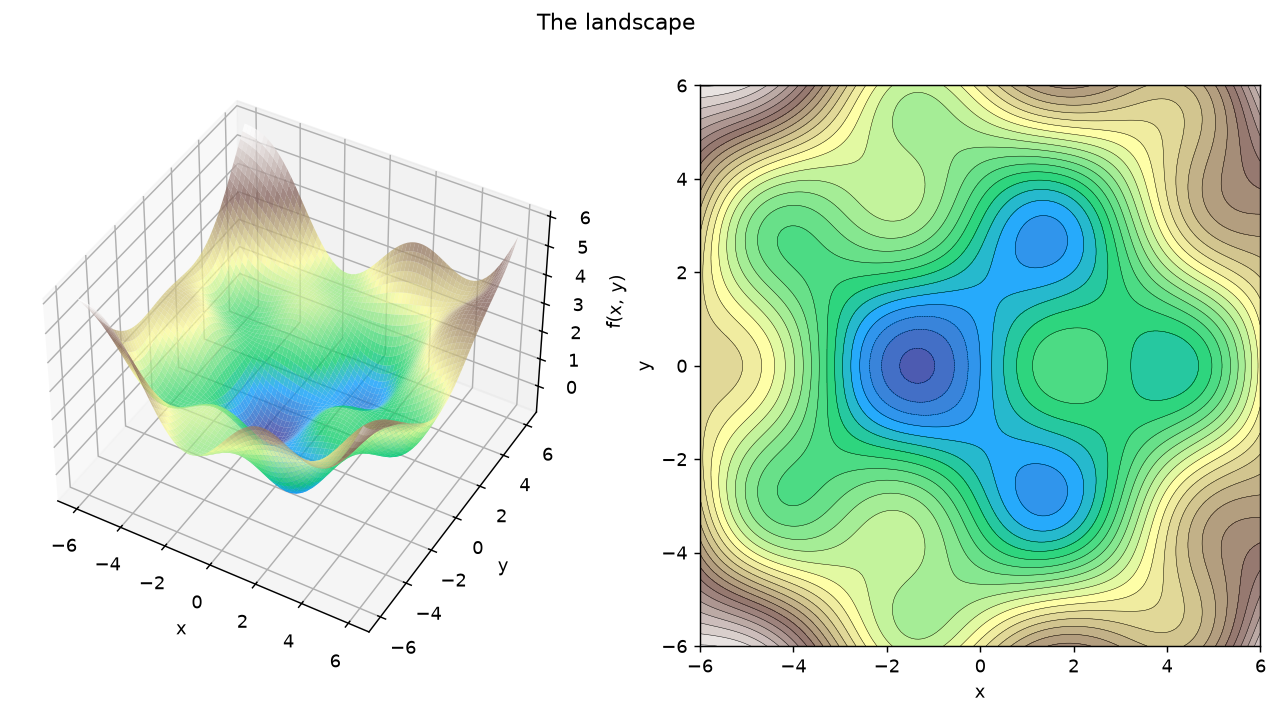
\includegraphics[width=0.94\textwidth]{landscape.png}
\end{center}

\begin{callout}{The algorithm: gradient descent (computational unit \S27.4)}
Given the gradient $\grad f$, a start $\vc{x}_0$, a learning rate $\eta>0$, a
tolerance $\tau$ and a cap on the number of steps:
\begin{enumerate}[label=\textbf{\arabic*.},leftmargin=2em,itemsep=2pt,topsep=2pt]
  \item Compute $\vc{g}=\grad f(\vc{x})$.
  \item If $\norm{\vc{g}}<\tau$, stop: the ground is flat, report success.
  \item Otherwise step downhill, $\vc{x}\leftarrow\vc{x}-\eta\,\vc{g}$, and go
        back to 1 --- unless the cap has been reached, in which case report
        failure.
\end{enumerate}
It works because $\grad f$ points in the direction of steepest ascent (vector
calculus unit \S8.3), so $-\grad f$ points steepest downhill. The learning rate
decides how far to go: too small and the marble crawls, too large and it
overshoots (computational unit \S25.4).
\end{callout}

\begin{task}[\texttt{grad\_f}]
Compute $\partial f/\partial x$ and $\partial f/\partial y$ by hand (vector
calculus unit \S6.3: hold the other variable constant). Write your derivation
in the report (R1), then code \texttt{grad\_f(p)} to return
$\grad f=[\,\partial f/\partial x,\ \partial f/\partial y\,]$ as a NumPy array.
\checkpoint{$\grad f(0,0)=[\,1,\ 0\,]$. \file{runproject1.py} also compares your gradient
with a numerical one (built from the limit definition) at $50$ random points;
the largest disagreement should be around $10^{-9}$. If it is anywhere near
$1$, a partial derivative is wrong.}
\end{task}

\begin{task}[\texttt{gradient\_descent}]
Write
\begin{center}
\texttt{gradient\_descent(grad, x0, lr, tol=1e-6, max\_iter=1000)}
\end{center}
following the box, taking at most \texttt{max\_iter} steps. Return
\texttt{path}, the list of every point visited starting with \texttt{x0}, and
\texttt{converged}, which is \texttt{True} if the test in step 2 passed.
\heads{Build each new point as a new array, as \texttt{x = x - lr * g} does,
or append a \emph{copy} of it to the path. Updating one array in place with
\texttt{x -= lr * g} would leave every entry of your path pointing at the same,
final, point.}
\checkpoint{\file{runproject1.py} first runs the example of computational unit \S27.2,
$f(x,y)=x^{2}+y^{2}$ from $[1,2]$ with $\eta=0.1$. The path begins $[1,2]$,
$[0.8,1.6]$, $[0.64,1.28]$, $[0.512,1.024]$, and converges after $69$ steps.
With $\eta=1$ it bounces between $[1,2]$ and $[-1,-2]$ forever, and after the
cap of $20$ steps it is back at $[1,2]$ with \texttt{converged} \texttt{False}
--- the row $\eta=1$ of the table in \S25.4.}
\end{task}

\begin{task}[Five marbles --- nothing to write]
\file{runproject1.py} drops five marbles with $\eta=0.3$ and reports where each one
settled, how deep its valley is, and how many steps it took.
\checkpoint{The first marble, dropped at $(0.5,0.5)$, settles at about
$(-1.353,\ 0)$ with $f\approx-0.830$ after $39$ steps.}
\watch{\texttt{python play.py marbles} shows all five rolling at once, on the
3-D surface and on the contour map.}
\end{task}

\begin{task}[Learning rates --- nothing to write]
From the single start $(3,\ 1.5)$ \file{runproject1.py} tries $\eta=0.01$, $0.1$, $0.5$,
$1$, $1.5$ and $2$, and reports which runs converged and how fast. Then it
drops one marble at $(-4,\ 4.6)$ twice, with $\eta=0.1$ and with $\eta=1.5$.
\watch{\texttt{python play.py rates} races those last two marbles.}
\end{task}

\subsection*{The report for Choice 3}

\begin{enumerate}[label=\textbf{R\arabic*.},leftmargin=2.6em,itemsep=6pt,topsep=4pt]
  \item \textbf{The gradient (Task 3.1).} Show your derivation of
        $\partial f/\partial x$ and $\partial f/\partial y$, naming the rule
        you use at each step. Then evaluate your gradient at $(0,0)$ by hand,
        and quote the largest disagreement with the numerical gradient that
        \file{runproject1.py} found.
  \item \textbf{Marbles and learning rates (Tasks 3.3--3.4).} Which marble
        found the deepest valley? Two marbles took about ten times as many
        steps as the others: look at the contour map near where they stopped
        and explain what is different about those valleys. Make a table of the
        learning-rate runs and explain each kind of behaviour you see. Finally,
        the marble at $(-4,\ 4.6)$ reached the deepest valley only with the
        larger learning rate. Is that a reason to use large learning rates?
\end{enumerate}

\noindent\textbf{Limits.} Write a short paragraph on the limits of gradient
descent: one thing it cannot do, or does badly, that you saw in this project,
and one more that you did not see here but would expect on real problems.
Computational unit \S26.2, ``What goes wrong'', is a good place to look.

%==============================================================================
\section*{Optional and ungraded}
%==============================================================================
\begin{itemize}[leftmargin=1.4em,itemsep=5pt,topsep=3pt]
  \item \textbf{Try another choice.} \texttt{python runproject1.py kmeans} runs
        Choice 2 whatever \texttt{TRACK} says, and likewise \texttt{knn},
        \texttt{descent}, or \texttt{all}. Only the choice named by
        \texttt{TRACK} is graded.
  \item \textbf{Paint by numbers} (Choice 2). Load a photo with
        \texttt{plt.imread}, treat every pixel as a point
        $[\text{red},\text{green},\text{blue}]$ in $\R^{3}$, run your
        \texttt{kmeans} with $k=8$ on a random sample of a few thousand pixels,
        and repaint every pixel with the colour of its nearest centre. Your
        \texttt{assign} works unchanged in $\R^{3}$. Why?
  \item \textbf{Make a GIF} (Choice 3). \texttt{viz.watch\_descent} takes a
        \texttt{save\_frames} argument that saves every frame as a picture; any
        GIF maker will stitch them together for your report.
\end{itemize}

\bigskip
\noindent\rule{\textwidth}{0.4pt}

\smallskip
\noindent{\small Questions about the project belong in the class Discord, where
everyone can see the answer. Questions about your own code are better brought to
office hours, Thursdays 3:00--4:00 PM in Kiely Hall 508. Please email ahead.}

\end{document}
